\begin{figure} 
	\centering
	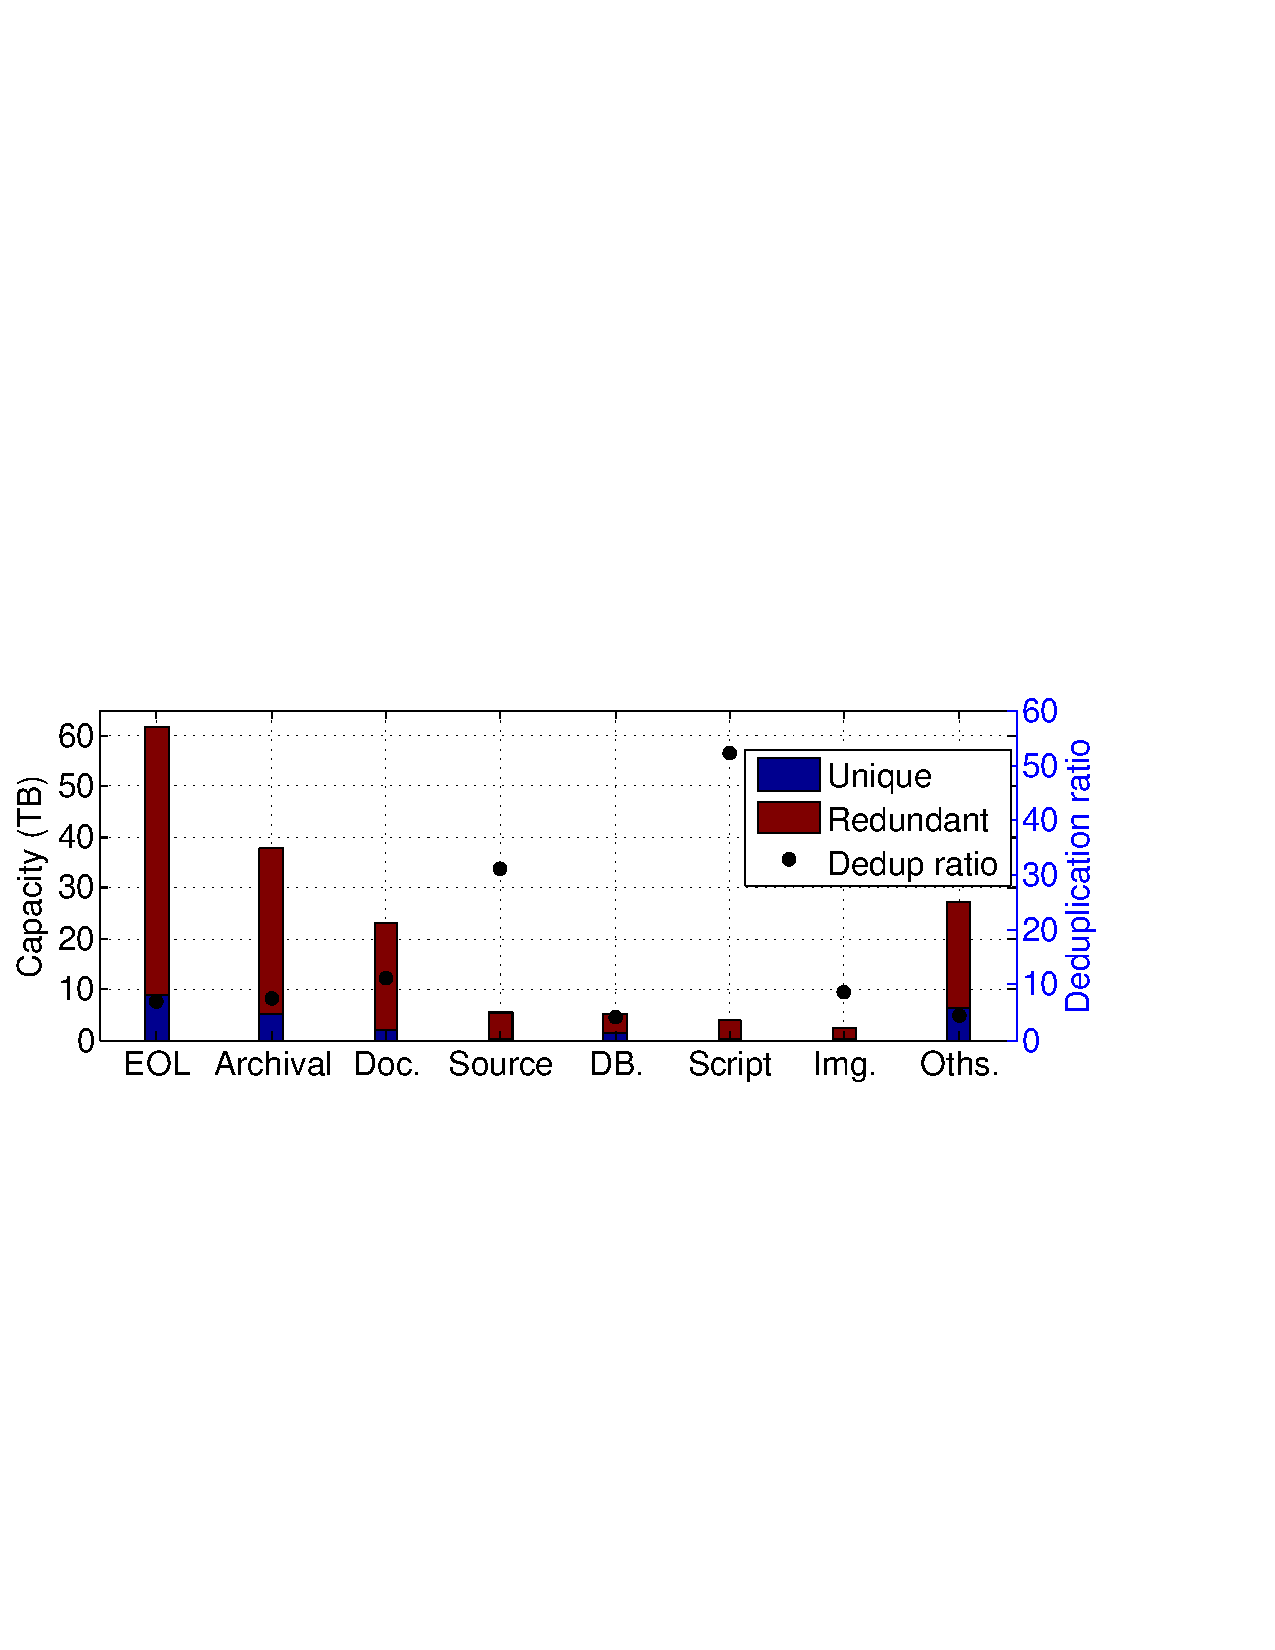
\includegraphics[width=0.45\textwidth]{graphs/dedup-overall} 
	\caption{Deduplication ratio for seven file classes---EOL, archival, documents, source code, database, scripts, images---and other files.
	Light bars indicate the original storage utilization while dark bars represent the capacity after removing redundant files.
	Dots shows the corresponding deduplication ratio.
%
%\VT{Can we stretch X axis to column width to have more space for X-axis labels?}\NZ{addressed}
%%
%\VT{Explain what blue and red bars mean here, as well as dots. Explain
%if dedup ratio is in terms of capacity or file counts.}\NZ{addressed}
%
} 
	\label{fig:dedup-overall} 
\end{figure}


